Section \ref{sec:challenges-control-rod} highlighted the poor performance of neutron diffusion
methods for calculating neutron fluxes near control rods. Strong neutron absorption in the control
rod region produces highly anisotropic neutron flux extending some distance outside the control
rod. Neutron transport methods, which retain angular dependence of the neutron flux in one way or
other, generally fare better than neutron diffusion methods with isotropic diffusion coefficients.
However, neutron transport methods are also generally more computationally expensive given the
increased dimensionality of the problem from the angular component. Piling this extra dimension on
top of the existing geometric and neutron energy group dimensions greatly multiplies the unknowns
to be solved in a system. Many past efforts have tried introducing transport correction techniques
to improve neutron flux and multiplication factor estimates with diffusion-based methods. Other
than control rod regions, these techniques also correct for homogenization error introduced from
spatial homogenization of fuel assemblies and other structures within a reactor core. They
invariably rely on neutron transport methods to generate transport corrections in the form of
corrected diffusion coefficients, boundary conditions, Eddington factors or discontinuity factors.

In this chapter, I propose a novel hybrid method for improving control rod modeling in neutron
diffusion solvers without spatial homogenization. In essence, the hybrid method involves applying
the $S_N$ discrete ordinates neutron transport method on subregions containing the control rod to
obtain transport corrected diffusion coefficients for the diffusion method on the entire problem
domain. 

Section \ref{sec:hybrid-theory} discusses the theoretical background for the hybrid $S_N$-Diffusion
method. Thereafter, Section * discusses some preliminary results of the hybrid method with a 1-D
finite difference implementation on a graphite-moderated system similar to the \gls{MSRE} design.

\section{Theory} \label{sec:hybrid-theory}

The proposed hybrid $S_N$-Diffusion method is a two-level, iterative method to improve the
accuracy of neutron diffusion solutions in reactor systems with highly neuutron-absorbing control
rod regions. In this discussion, I will focus on the 1-D, time-independent implementation of the
hybrid method.

The discrete ordinates ($S_N$) method for solving the multigroup neutron transport equation
(Eq. \ref{eq:mg-bte}) discretizes the continuous angular directional phase space into a finite
number of discrete angular intervals (ordinates). The set of distinct direction variables
$\hat{\Omega}_n$ representing the discrete ordinates is typically chosen in conjunction with a
compatible quadrature set to replace the integrals across the continuous solid angles
$\hat{\Omega}$ with quadrature approximations. The multigroup, discrete ordinates ($S_N$
approximation) form of the 1-D, time-independent neutron transport equation with the Gauss-Legendre
quadrature set is given as:
%
\begin{align}
  \mu_n \frac{d}{dx}\Psi_g(x, \mu_n) + \Sigma_{t,g}(x)&\Psi_g(x, \mu_n) -
\sum^G_{g'=1} \sum^N_{n'=1} \sum^L_{l=0} \frac{\left(2l+1\right)}{2}
\Sigma^{g'\rightarrow g}_{s,l}(x) P_l(\mu_{n'} - \mu_n)
w_{n'}\Psi_{g'}(x,\mu_{n'}) \nonumber \\
  &= \sum^G_{g'=1} \frac{\chi_g}{2} \nu\Sigma_{f,g}(x) \phi_{g'}(x) + S_g(x,\mu_n)
  \shortintertext{where}
  \mu_n &= \mbox{ cosine of $\hat{\Omega}_n$ relative to the $x$-axis,} \nonumber \\
  \Psi_g(x,\mu_n) &= \mbox{ neutron angular flux along $\mu_n$ in group $g$,} \nonumber \\
%  g &= \mbox{ neutron energy group index, ranging from 1 to G,} \nonumber \\
%  \Sigma_{t,g}(x) &= \mbox{ macroscopic total cross section of neutrons in group $g$,} \nonumber \\
%  G &= \mbox{ total number of energy groups,} \nonumber \\
%  n &= \mbox{ discrete ordinate index,} \nonumber \\
%  N &= \mbox{ total number of discrete ordinates,} \nonumber \\
  l &= \mbox{ Legendre order,} \nonumber \\
  L &= \mbox{ highest Legendre order,} \nonumber \\
  \Sigma^{g'\rightarrow g}_{s,l}(x) &= \mbox{ $l$-th Legendre expansion of the macroscopic
scattering} \nonumber \\
  &\mbox{ cross section from group $g'$ to $g$,} \nonumber \\
  P_l &= \mbox{ $l$-th Legendre polynomial,} \nonumber \\
  w_{n'} &= \mbox{ $n'$-th quadrature weight,} \nonumber \\
%  \chi_g &= \mbox{ fission neutron spectrum in group $g$,} \nonumber \\
%  \nu &= \mbox{ neutrons produced per fission reaction,} \nonumber \\
%  \Sigma_{f,g}(x) &= \mbox{ macroscopic fission cross sectionof neutrons in group $g$,} \nonumber \\
%  \phi_{g'}(x) &= \mbox{ scalar neutron flux in group $g$,} \nonumber \\
%  S_g(x,\mu_n) &= \mbox{ external neutron source in group $g$.} \nonumber
\end{align}
%
The neutron scalar flux and current can be retrieved by calculating the 0th and 1st Legendre moments
as follows:
%
\begin{align}
  \phi_g(x) &= \frac{1}{2} \int^1_{-1} d\mu\ \Psi_g(x,\mu) = \frac{1}{2} \sum^N_{n=1} w_n
\Psi_g(x,\mu_n)
  \shortintertext{and}
  J_g(x) &= \frac{1}{2} \int^1_{-1} d\mu\ \mu\Psi_g(x,\mu) = \frac{1}{2} \sum^N_{n=1} w_n
\mu_n \Psi_g(x,\mu_n)
\end{align}

The 1-D form of the multigroup time-independent neutron diffusion equations (Eq. \ref{eq:mg-diff})
is given as:
%
\begin{align}
  -\frac{d}{dx} D_g(x) \frac{d}{dx} \phi_g(x) + \Sigma_{t,g}(x) \phi_g(x) &= \sum^G_{g'=1}\left[
  \Sigma_s^{g'\rightarrow g}(x)\phi_{g'}(x) + \chi_g\nu\Sigma_{f,g'}\phi_{g'}(x)\right] + S_g(x)
  \label{eq:1d-diff}
  \shortintertext{where}
    D_g(x) &= \frac{1}{3 \Sigma_{tr}(x)} = \mbox{ neutron diffusion coefficient for group }g.
  \nonumber
\end{align}

\subsection{Spatially Varying Diffusion Coefficients} \label{sec:svdc}

The conventional approach for determining diffusion coefficients based on the $P_1$ approximation
for each subregion involves running a high-fidelity neutron transport to tally region-wide
estimates of the neutron transport cross section. In essence, a single value represents the
isotropic diffusion coefficient for the entire (e.g. fuel, moderator, reflector) subregion.
However, as discussed in Section \ref{sec:challenges-control-rod}, the neutron diffusion equation
is only valid in regions of high scattering-to-absorption ratios and away from interfaces to
neighboring media with highly dissimilar neutronic properties.

In the hybrid $S_N$-Diffusion method, I propose replacing the conventional $P_1$-based
diffusion coefficients with an alternate formulation which incorporates point-wise corrections
to the neutron diffusion flux solution from the $S_N$-derived flux solution as follows:
%
\begin{align}
  D^s_g(x) &= -J^{tr}_g(x)\bigg/\frac{d\phi^{tr}_g(x)}{dx}. \label{eq:svdc}
\end{align}
%
where $D^s$ is the \glspl{SVDC}, and the $tr$ superscript denotes neutron current and scalar flux
solutions from the $S_N$ method.
The basic form of this equation is Fick's first law of diffusion. The end result is a diffusion
coefficient variable that varies in space even within a subregion and provides pointwise
corrections to closely match the diffusion flux solution to the $S_N$ flux solution.

Pounders \& Rahnema \cite{pounders_diffusion_2009} demonstrated the effectiveness of applying
point-wise corrections derived from analytical or Monte Carlo reference flux solutions. Compared
with conventional $P_1$-based out-scatter and flux-limited approximations of the diffusion
coefficient, their \textit{high-order empirical diffusion coefficient} showed superior agreement
with the reference flux solutions. Their formulation for these piecewise-constant empirical
diffusion coefficients in Eq. \ref{eq:emp} is similar to the formulation for \glspl{SVDC} in Eq.
\ref{eq:svdc} after finite difference discretization. They recognized that the volume
averaging for piecewise-constant coefficients will introduce some truncation error if the flux is
non-linear within each mesh element. This design choice may be due to an intention to retain the
diffusion coefficient as a constant in the $\frac{d}{dx}D\frac{d\phi}{dx}$ term of the neutron
diffusion equation (Eq. \ref{eq:1d-diff}).

Unlike their approach, the \gls{SVDC} formulation in Eq. \ref{eq:svdc} allows for continuously
varying diffusion coefficients to reduce truncation error. In practice, the discretization order of
\gls{SVDC} variables in a numerical calculation would follow the discretization order of the
reference flux solution. This formulation introduces a minor change to the finite difference
implementation of the second-order diffusion term to specifically handle spatial derivatives of the
diffusion coefficient, but the finite element implementation will see no change as the second-order
diffusion term is commonly treated with integration-by-parts to reduce it to a first-order
differential term. Refer to Section * for a numerical implementation of a finite difference neutron
diffusion solver with support for \glspl{SVDC}.

\begin{figure}[htb!]
  \centering
  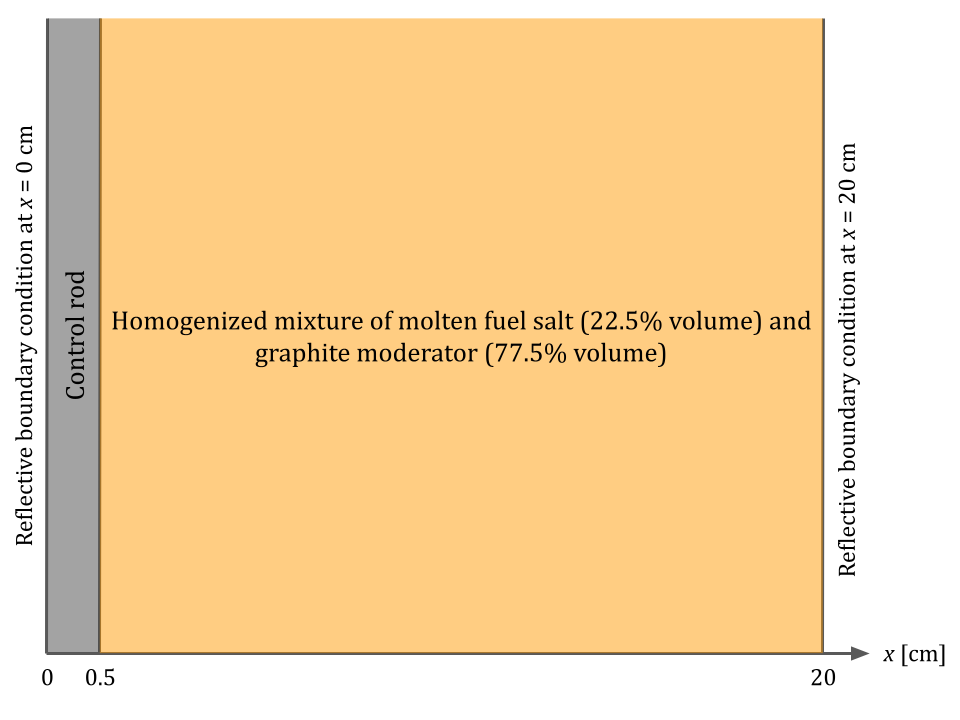
\includegraphics[width=.7\columnwidth]{case-0-geometry}
  \caption{A 1-D, two-region system containing a 0.5 cm-thick control rod and a 24.5 cm-thick
    homogeneous mixture of molten fuel salt and graphite moderator. Reflective boundary conditions
    are applied on both ends.}
  \label{fig:case-0-geom}
\end{figure}

To facilitate the following demonstration of a neutron diffusion calculation with \glspl{SVDC},
consider a 1-D, two-region system consisting of a highly neutron absorbing material and a neutron
multiplying region with reflective boundary conditions on both ends (Figure \ref{fig:case-0-geom}).
The material specifications are taken from the control rod, molten fuel salt, and graphite
moderator compositions of the \gls{MSRE} \cite{robertson_msre_1965}. The molten fuel salt and
graphite regions are homogenized to minimize discrepancies arising from geometrical heterogeneity.
The group constant input data for the diffusion and $S_N$ solvers (e.g. cross sections, fission
spectra, etc.) were sampled at 900 K the OpenMC Monte Carlo neutronics software. The neutron energy
spectrum is condensed into two discrete groups bounded at $10^{-5}$, $10^0$, and $10^8$ eV.

I solved for the neutron flux in this system using the following set of numerical solvers:
%
\begin{enumerate}
  \item Diffusion solver with $P_1$ flux-limited diffusion coefficients generated directly from the
    OpenMC calculation.
  \item $S_4$ solver with up to 1st-order Legendre expansions of the group-to-group neutron
    scattering cross sections.
  \item Diffusion solver with \glspl{SVDC} generated from the prior $S_4$ flux solution.
\end{enumerate}
%
All other relevant group constants are identical and unchanged from the original dataset generated
using OpenMC. I implemented the diffusion solvers using the finite difference method and the $S_N$
solver using a diamond-differenced transport sweep method in Python. For brevity, further numerical
implementation details of these solvers are deferred to Section \ref{sec:implementation}.

\begin{figure}[htb!]
  \centering
  \begin{subfigure}[b]{.49\textwidth}
    \centering
    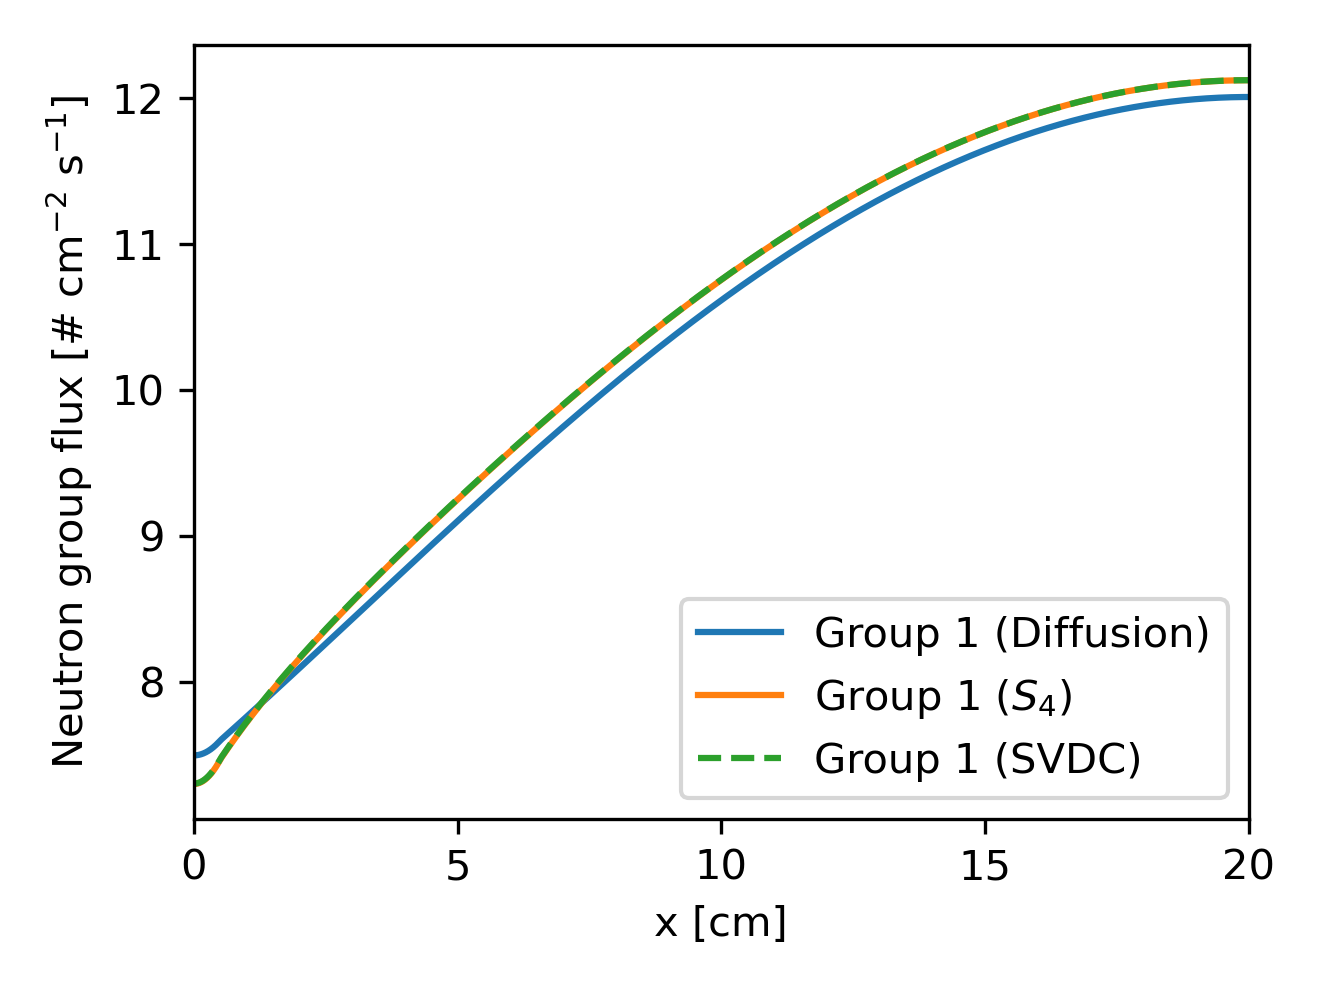
\includegraphics[width=\textwidth]{case-0-group-1-flux}
    \caption{Group 1 flux}
    \label{fig:c0g1flux}
  \end{subfigure}
  \hfill
  \begin{subfigure}[b]{.49\textwidth}
    \centering
    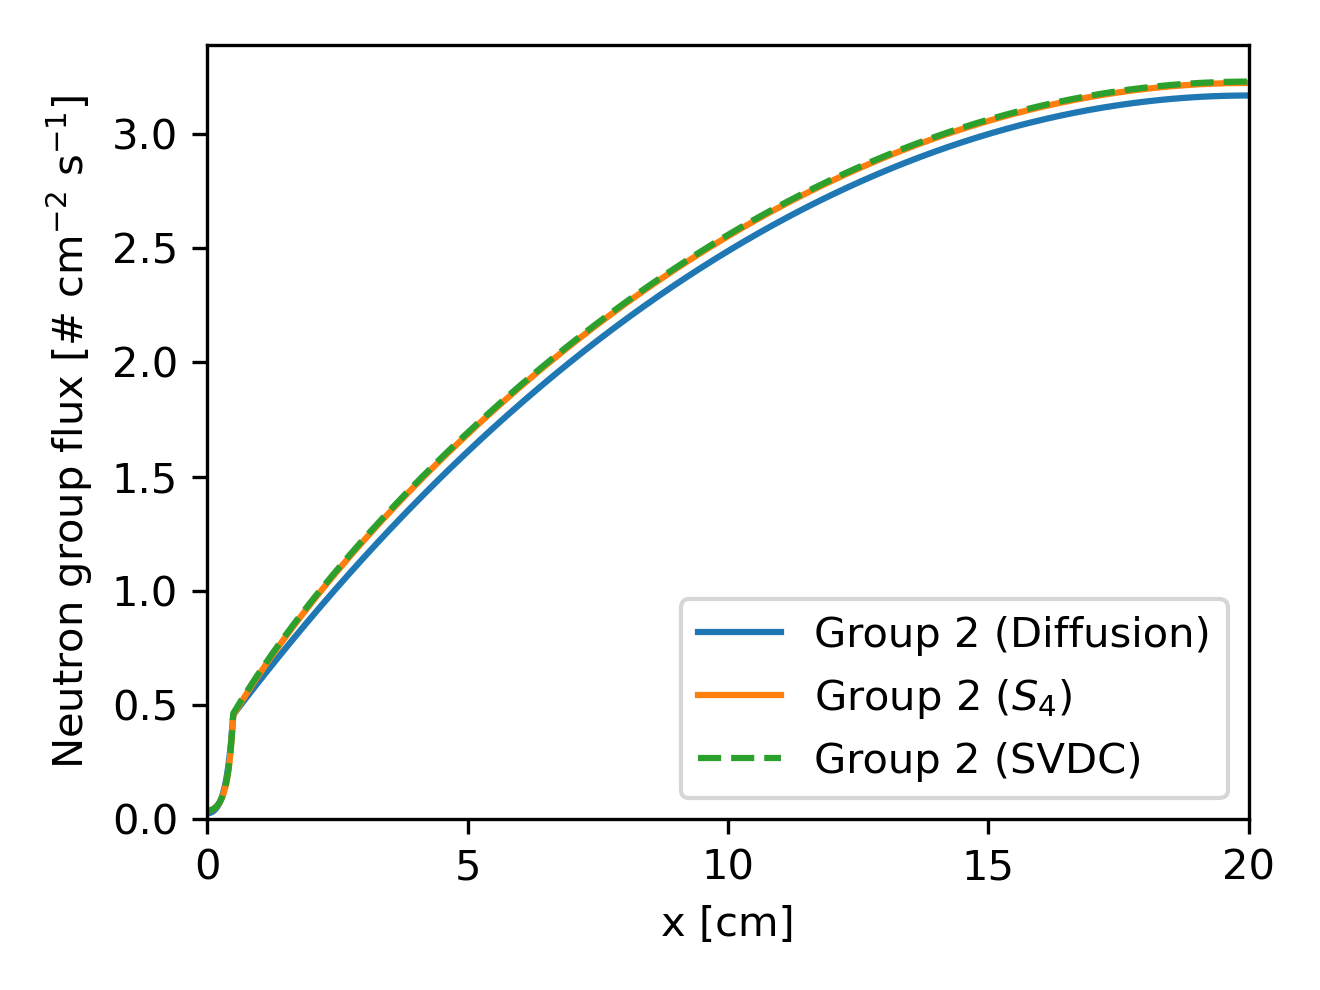
\includegraphics[width=\textwidth]{case-0-group-2-flux}
    \caption{Group 2 flux}
    \label{fig:c0g2flux}
  \end{subfigure}
  \caption{Neutron group flux solutions of the 1-D, two-region system from the diffusion, $S_4$,
    and diffusion-\gls{SVDC} solvers.}
  \label{fig:c0flux}
\end{figure}
%
\begin{figure}[htb!]
  \centering
  \begin{subfigure}[b]{.49\textwidth}
    \centering
    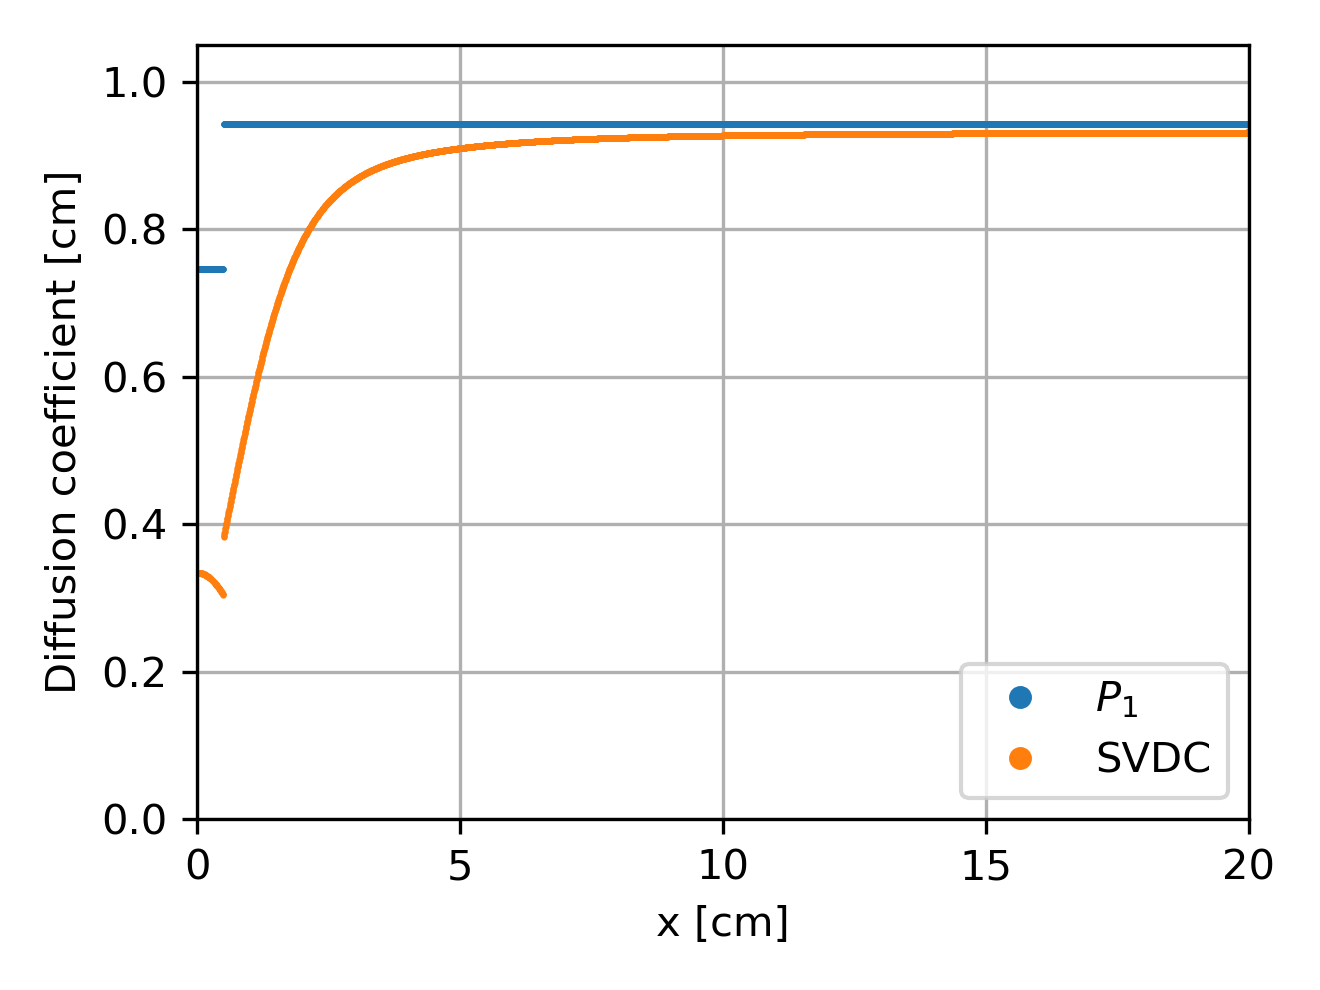
\includegraphics[width=\textwidth]{case-0-group-1-diffcoef}
    \caption{Group 1 diffusion coefficients}
    \label{fig:c0g1diffcoef}
  \end{subfigure}
  \hfill
  \begin{subfigure}[b]{.49\textwidth}
    \centering
    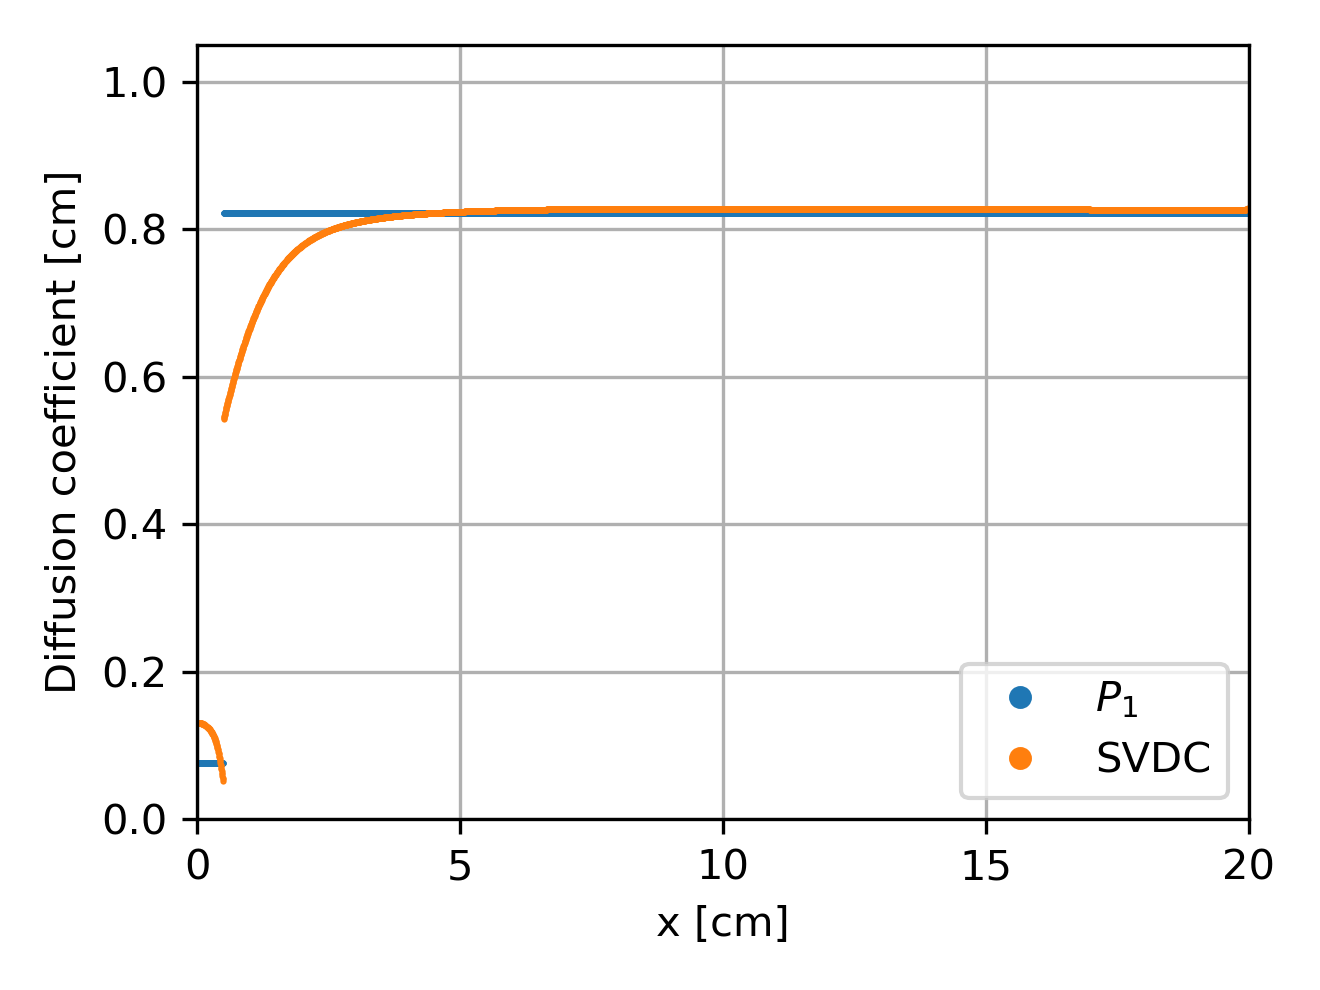
\includegraphics[width=\textwidth]{case-0-group-2-diffcoef}
    \caption{Group 2 diffusion coefficients}
    \label{fig:c0g2diffcoef}
  \end{subfigure}
  \caption{$P_1$-based flux-limited diffusion coefficients and \glspl{SVDC} in the 1-D, two-region
  system.}
  \label{fig:c0flux}
\end{figure}

Figure \ref{fig:c0flux} shows the group 1 and 2 neutron fluxes from the diffusion-$P_1$, $S_4$, and
diffusion-\gls{SVDC} solvers with a fixed mesh size of 0.005 cm. The OpenMC flux solution is
omitted because the purpose of this exercise is to demonstrate the effectiveness of \glspl{SVDC}
in reproducing a $S_N$ flux solution. As expected, the diffusion-$P_1$ flux solution deviates from
the $S_4$ flux solution while the diffusion-\gls{SVDC} flux solution shows significantly better
agreement with the $S_4$ flux solution. As shown in Table \ref{table:c0k}, $k$ estimate from the
diffusion-\gls{SVDC} solver (0.79594) is also closer to the $k$ estimate from the $S_4$ solver
(0.79467) than the diffusion-$P_1$ solver (0.78185).

\begin{table}[tb!]
  \centering
  \caption{Multiplication factor $k$ estimates from the diffusion-$P_1$, $S_4$, and
  diffusion-\gls{SVDC} solvers and the absolute difference relative to the $S_4$ estimate.}
  \begin{tabular}{l S S}
    \toprule
    Solver type & {$k$} & {Diff.} \\
    \midrule
    Diffusion-$P_1$ & 0.60976 & -0.01448 \\
    $S_4$ & 0.62424 & {-} \\
    Diffusion-\gls{SVDC} & 0.62554 & +0.00130 \\
    % OpenMC & {0.64604 +/- 0.00051} & {-} \\
    \bottomrule
  \end{tabular}
  \label{table:c0k}
\end{table}

Comparing the $P_1$-based diffusion coefficients and \glspl{SVDC} in Figure *, both quantities
agree closely in the bulk fuel salt region far away from the control rod region. This observation
supports the validity of the neutron diffusion method with $P_1$ approximations in a homogeneous
medium with high scattering-to-absorption ratios. Moving towards the control rod region, the
\glspl{SVDC} deviate from the $P_1$-based diffusion coefficients as the prerequisite assumptions
for diffusion theory do not hold anymore.

Thus far, this method is trivial and completely redundant because it requires a priori
knowledge of the true flux solution or at least a highly accurate solution calculated using neutron
transport methods. While existing workflows for diffusion-based methods already require
computationally intensive neutron transport simulations to generate input data for the neutron
diffusion equation, this preprocessing step (known as \textit{group constant generation}) requires
a fixed number of neutron transport simulations. For instance, $P_1$-based diffusion coefficients
may be generated at various reactor temperatures. In the subsequent multiphysics reactor analysis,
these diffusion coefficient values may be interpolated for diffusion coefficient estimates at other
temperatures within the validity range. On the other hand, \glspl{SVDC} will likely need to be
dynamically generated at every timestep, such as with a two-level iterative scheme consisting of a
high-level $S_N$ neutron transport calculation and a low-level neutron diffusion calculation.

The nature of \glspl{SVDC} as empirical, pointwise corrections for
the diffusion equation makes it highly dependent on the neutron flux gradient, and
susceptible to greater variations than region-wide estimates for $P_1$-based diffusion
coefficients. Compared to \glspl{SVDC}, $P_1$ diffusion coefficients behave much more like
intrinsic material properties as their definitions are largely tied to material cross sections.
Variations in $P_1$ diffusion coefficients largely arise from changes in the neutron energy
spectrum with no direct contribution from proximity to material interfaces (geometrical
heterogeneity).

Another significant challenge of \glspl{SVDC} and the high-order empirical diffusion coefficients
involves their determination near neutron flux peaks. The neutron currents and
flux gradients in the numerator and denominator of Eq. \ref{eq:svdc} generally do not go to zero at
the same point, resulting in very large positive or negative diffusion coefficient values when the
flux gradient is close or equal to zero. Pounders \& Rahnema tackled this issue by using
larger mesh sizes with which to calculate their empirical diffusion coefficients. However, their
remedy significantly worsens flux accuracy in regions with steep, non-linear flux such as in
control rods. I will investigate and find an alternative solution for this issue in the
implementation of \glspl{SVDC} in the proposed work.

\subsection{Hybrid $S_N$-Diffusion Method} \{sec:hybrid-method}

In order to reduce the computational cost of the high-level $S_N$ calculation, I propose reducing
the problem domain of the $S_N$ method to the control rod and its vicinity. Consequently, the
hybrid $S_N$-Diffusion method can retain accurate neutron flux estimates around the control rod
region from the $S_N$ method while making significant savings in computational cost by treating the
majority of the reactor geometry with the neutron diffusion method. Henceforth, I shall refer to
the $S_N$ calculation or method on the reduced problem domain as the $S_N$ \textit{subproblem} or
\textit{subsolver} accordingly. The problem domains of the neutron diffusion and $S_N$ calculations
are defined as $\Omega^d$ and $\Omega^d_1$, respectively, where $\Omega^d_1 \subseteq \Omega^d$.
The process is as follows:
%
%\begin{algorithm}
%  \caption{Hybrid $S_N$-Diffusion algorithm \label{alg:hybrid}}
%  \DontPrintSemicolon
%  \KwData{Material group constants and mesh of problem domain $\Omega^d$.}
%  \KwResult{Improved flux $\phi$ and multiplication factor $k$ estimates.}
%  \BlankLine
%  Initialize $\phi_g^0$, $k^0$, $D_g^0=D_g^{P_1}$; $m=0$\;
%  \While{$\epsilon_\phi > tol_\phi$ or $\epsilon_k > tol_k$}{
%    $m = m+1$\;
%    Solve the neutron diffusion equations for $\phi_g^m$ and $k^m$ using $D_g$ in domain
%    $\Omega^d$.\;
%    Update $\epsilon_\phi = ||\phi_g^m-\phi_g^{m-1}||_2/G/n$ where $G=$ total no. of groups and
%    $n=$ total no. of mesh elements.\;
%    Calculate neutron current boundary conditions along subdomain boundaries $\partial\Omega^d_1$
%    using $\phi_g^m$ and $D_g$, where $\Omega^d_1 \subset \Omega^d$
%  }
%\end{algorithm}
%
\begin{enumerate}
  \item Start with an initial neutron diffusion calculation in $\Omega^d$ with conventional $P_1$
    diffusion coefficients and other standard group constants (e.g. neutron cross sections).
  \item Use the neutron diffusion flux estimates in $\Omega^d_1$ and current estimates along
    $\partial \Omega^d_1$ as initial and boundary conditions for the $S_N$ subsolver.
  \item With the $S_N$ subsolver, calculate an improved neutron flux solution in $\Omega^d_1$ which
    contains the control rod region and its immediate vicinity.
  \item Calculate \glspl{SVDC} using the $S_N$ flux solution and Eq. \ref{eq:svdc}.
  \item Pass the \glspl{SVDC} to the neutron diffusion solver to replace the conventional
    $P_1$ diffusion coefficients within the regions that overlap with the $S_N$ solver problem
    domain.
  \item Run another neutron diffusion calculation with the \glspl{SVDC} within the overlapping
    domain.
  \item Pass the new neutron diffusion flux and current solutions to the $S_N$ subsolver.
  \item Iterate until convergence is reached by meeting pre-defined convergence tolerance values.
\end{enumerate}

The main challenge lies in determining appropriate boundary conditions for the $S_N$ subproblem.
Given that we want to limit the $S_N$ subproblem domain to the control rod
region and its immediate vicinity, the $S_N$ subproblem boundaries should lie well within
the reactor geometry. However, there is currently no feasible method of generating accurate
boundary fluxes for an $S_N$ solver from a neutron diffusion flux solution. In 1-D, the standard
$S_N$ method requires N/2 incoming flux boundary parameters per boundary mesh point for the N/2
neutron angular fluxes flowing inwards. The neutron diffusion method can produce at most one
independent parameter per mesh point; this parameter is the $P_1$ neutron forward/backward current
as follows:
%
\begin{align}
  J_{g,\pm} &= \frac{\phi_g}{4} \mp \frac{D_g}{2}\frac{d\phi_g}{dx}
  \shortintertext{where}
  J_{g,\pm} &= \mbox{ neutron forward/backward current of group }g. \nonumber \\
\end{align}
%
For now, I will assume that all N/2 angular fluxes are equal in magnitude, i.e. the flux is
isotropic throughout the half-sphere pointing into the $S_N$ subproblem domain. As a consequence,
the $S_N$ subsolver yields an inaccurate flux solution.

To resolve this issue, I posit the following hypothesis: \textit{If there exists a highly
neutron-absorbing control rod region within the $S_N$ subproblem domain $\Omega^d_1$ and the $S_N$
subproblem boundary $\partial\Omega^d_1$ lies several neutron mean free paths away from this
region, the \gls{SVDC} values calculated near the control rod region (using the $S_N$ subsolver
with half-sphere isotropic boundary conditions) will tend to the actual flux gradient solution
(using a reference $S_N$ calculation across the entire problem domain $\Omega^d$).} In other words,
while suboptimal boundary conditions may induce inaccurate \gls{SVDC} values near the $\partial
\Omega^d_1$ subdomain boundaries, the \gls{SVDC} values further from $\partial\Omega^d_1$ are very
weakly dependent on the boundary conditions.

I will use the same 1D, two-region system described in Section \ref{sec:svdc} (Figure
\ref{fig:case-0-geom}) to test my hypothesis and demonstrate the hybrid $S_N$-diffusion method.
$\Omega^d_1$ is defined as the region spanning from $x=0$ cm to $x=17.5$ cm. Note that
this region is a subdomain of the entire domain spanning from $x=0$ cm to $x=20$ cm.

Once again, the numerical implementation details are deferred to Section \ref{sec:implementation}.

Therefore, for a reactor system such as an \gls{MSR} which consists of mostly highly scattering
regions, we can set up a subproblem domain which covers a reasonably small fraction of the entire
reactor geometry. 

\section{Preliminary Work} \label{sec:preliminary}

\subsection{Numerical Implementation} \label{sec:implementation}

\subsection{Description of 1-D Models}

\subsection{Results}
